\chapter{Experiments and results}
\label{sec:experiments}

In this chapter, several novel SOH estimation procedures are introduced, each consisting in a combination of one feature extraction method followed by one regression model. Synthetic and real datasets, described in chapters \ref{sec:ev_model_ds_gen} and \ref{sec:aviloo_ds} respectively, are used to train and validate regression models for the SOH estimation, and finally to test their performances.

\section{Data preprocessing}
\label{sec:ds_preprocessing}
Several preprocessing steps have been performed on the two datasets, before using them for training and testing purposes. The two preprocessing pipelines are described in the following sections.

\subsection{Synthetic dataset}
\label{sec:synth_preprocessing}
The two synthetic datasets generated in sec. \ref{sec:ds_gen} have been used to train the proposed SOH estimation procedures and to evaluate their performances. The following preprocessing steps have been performed on each driving session of the two datasets:
\begin{enumerate}
    \item Filter out signals other than voltage, current and SOC.
    \item Set the first voltage and SOC measurements by backward linear interpolation:
    \begin{align}
        \text{V}(0) &= \frac{\text{V}(t_2)-\text{V}(t_1)}{t_2-t_1}(-t_1)+\text{V}(t_1)\\
        \text{SOC}(0) &= \frac{\text{SOC}(t_2)-\text{SOC}(t_1)}{t_2-t_1}(-t_1)+\text{SOC}(t_1)
    \end{align}
    where $t_1$ and $t_2$ are respectively the second and third timestamp at which signals were sampled\footnote{we set $\text{\texttt{sampling\_rate}} = 0.2$ s, so $t_1=0.2$ s and $t_2=0.4$ s.\label{note:sampling_rate}}. This is done in order to address a bug in Simulink's GBM block (sec. \ref{sec:battery_pack}) which gives incorrect voltage and SOC measurements at the beginning of the simulation.
    \item Format data into a multi-index Pandas dataframe, attaching the SOH value associated to the current driving session and a short identifier for the name of the drive cycle.
\end{enumerate}
The preprocessed driving sessions are then concatenated into a single dataset. At this point, each dataset consists of 315 driving sessions from half an hour to several hours long.

Each driving session is then split up into several non-overlapping 5-minute-long time windows which inherit the SOH value associated to that session. The time window extraction algorithm is reported in appendix \ref{sec:tw_extr_alg}. A total of $10192$ time windows are extracted from the e-up! dataset, and a total of $24224$ from the e-Golf dataset. The data associated to each time window can be viewed as a multivariate time series with $C=3$ channels (V, I, SOC) and length $T=1500$ (i.e. 300 s $\times$ 5 measurements/s), therefore the resulting datasets of extracted time windows are time series datasets (def. \ref{def:ts_ds}) with $N_\text{e-up!}=10192$ and $N_\text{e-Golf}=24224$ samples respectively.

Since synthetic data will be used both for training regression models and testing them, each of the two time windows datasets is randomly split into a training set (80\% of the time windows) and a test set (20\%). Time windows are sampled in a stratified fashion, so that the distribution of different SOH levels in each subset is the same as in the original dataset.

Finally, standardization is applied to each signal, both in training and test set. Namely, the measurements $s_1,\dots,s_T$ of each signal are transformed to:
\begin{equation}
    z_i = \frac{s_i-\bar{\mathbf{s}}^\text{(train)}}{\hat{\sigma}_\mathbf{s}^\text{(train)}}
\label{eq:standardization}
\end{equation}
where $\bar{\mathbf{s}}^\text{(train)}$ and $\hat{\sigma}_\mathbf{s}^\text{(train)}$ are respectively the sample mean and sample standard deviation of the signal measurements in the training set. Computing the mean and standard deviation with respect to only the training set avoids data leakage from test data, which must be kept unseen until the end of the training phase.

We can convert each time series dataset to a static one by extracting relevant features from each time window. Feature extraction may be performed in a variety of ways, outlined in sec. \ref{sec:feature_extraction}.

\subsection{Real dataset}
\label{sec:aviloo_preprocessing}
Real field data (sec. \ref{sec:aviloo_ds_exploration}) has been used to evaluate the performances of the SOH estimation procedures, previously trained on synthetic data. The following preprocessing steps have been performed on each driving session of the two real datasets:
\begin{enumerate}
    \item Filter out signals other than voltage, current and SOC.
    \item Resample signals through linear interpolation with the same sampling rate specified for the synthetic dataset (sec. \ref{sec:ds_gen}). This is done in order to achieve a common time base for all signals.
    \item Format data into a multi-index Pandas dataframe, attaching the SOH value associated to the current driving session and a short identifier for the name of the drive cycle. Each signal will have its own column.
\end{enumerate}
The preprocessed driving sessions are concatenated into a single dataset. The synthetic and real datasets are now formatted all in the same way.

Time windows are then extracted from driving sessions, as already described in sec. \ref{sec:synth_preprocessing}. $N_\text{e-up!}=164$ and $N_\text{e-Golf}=1445$ samples are extracted in total. Similarly, signal standardization (eq. \ref{eq:standardization}) is applied at the end, reusing the already computed $\bar{\mathbf{s}}^\text{(train)}$ and $\hat{\sigma}_\mathbf{s}^\text{(train)}$. As already done for synthetic data, feature extraction is also performed on the two resulting real time windows datasets (sec. \ref{sec:feature_extraction}).

\section{Feature extraction}
\label{sec:feature_extraction}
Feature extraction provides a static representation for each time series dataset, making it easier to train regression models. To perform feature extraction, three approaches may be taken:
\begin{itemize}
    \item \textsc{MiniRocket}'s feature extraction for multivariate time series (sec. \ref{sec:multivariate-minirocket})
    \item OLS feature extraction (sec. \ref{sec:ols})
    \item Theil-Sen feature extraction (sec. \ref{sec:theil-sen})
\end{itemize}
Each approach has its pros and cons. \textsc{MiniRocket} extracts 9,996 features from each time series and is considered the state-of-the-art for TSER problems. However, it needs to be fit to training data in order to use it; moreover, its transform operation is computationally expensive, as almost 10,000 convolutions per time window need to be computed. OLS feature extraction\footnote{The key idea that motivates feature extraction based on OLS and Theil-Sen linear regression to time windows of EV monitoring data has been discussed in sec. \ref{sec:my_method}.\label{note:ols_ts_feat_extr}} generates 3 features per time series, does not need to be fit on training data and is computationally cheaper than \textsc{MiniRocket}. However, it is not robust to outliers in the V-I-SOC space. Theil-Sen feature extraction\footref{note:ols_ts_feat_extr} is similar to OLS, but is more robust to outliers. However, it is more computationally demanding than both OLS and \textsc{MiniRocket}.

Due to the huge number of features extracted by \textsc{MiniRocket}, PCA is applied to \textsc{MiniRocket}-transformed datasets. By visualizing the scree plot for the two synthetic training sets (fig. \ref{fig:scree_plot}), we observe that with just 32 features out of the original 9,996 we can explain over 90\% of the total variance in the data. A different PCA problem is solved for each of the two synthetic training sets. The first 32 principal components of the training sets are then used for all PCA transforms. Since PCA requires standardized data, time series data transformed through \textsc{MiniRocket} is standardized before the PCA transform\footnote{with sample mean and sample standard deviation defined by the synthetic training sets\label{note:pca_standardization}}. Furthermore, the PCA transform does not necessarily output standardized data, so standardization is applied also after every PCA transform\footref{note:pca_standardization}.

\begin{figure}[hbt!]
    \centering
    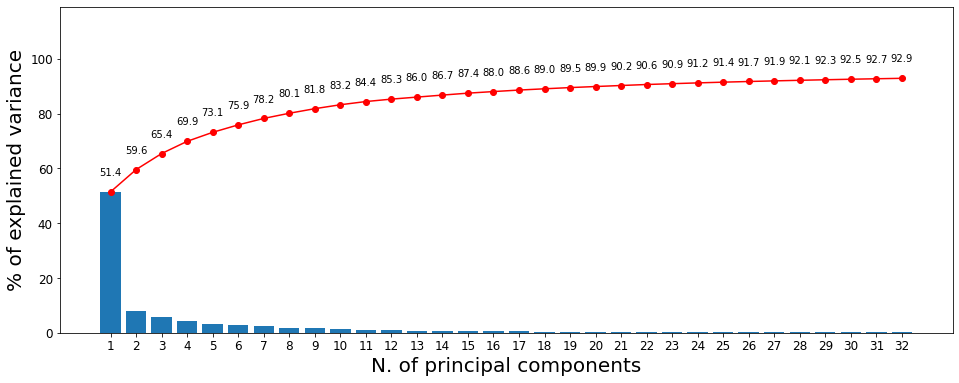
\includegraphics[width=\textwidth]{images/scree_plot}
    \caption[Scree plot for the \textsc{MiniRocket}-transformed e-Golf training set]{Scree plot for the \textsc{MiniRocket}-transformed e-Golf training set. The scree plot for the e-up! training set is very similar, thus it is not reported.}
    \label{fig:scree_plot}
\end{figure}




\section{Training regression models}
\label{sec:regr_model_training}
Several regression models can be selected for predicting the SOH from a transformed time window. In sec. \ref{sec:regr_models}, three models were discussed:
\begin{itemize}
    \item Ridge regression via SGD (RR, sec. \ref{sec:ridge})
    \item Random forest (RF, sec. \ref{sec:random_forest})
    \item Feed-forward neural network (NN, sec. \ref{sec:neural_network})
\end{itemize}
Three instances of each model are trained, one for each feature extraction method (for a total of 9 regression models per EV model). The training set used is the one introduced in sec. \ref{sec:synth_preprocessing}. Grid search with 5-fold cross-validation was performed to tune some of the hyperparameters of ridge regression and random forest models. The neural network hyperparameters were instead tuned by "trial and error", due to the higher computational cost of training such models; 10\% of the training set was set aside before training the neural network, to validate its performances at the end of each epoch. The optimal hyperparameters found are reported in appendix \ref{sec:hyperparameter tuning}. The workstation used to perform the training has the following specifications: Intel Xeon W-2155 CPU @ 3.30 GHz (10 cores, 20 threads), 64GB RAM, NVIDIA Quadro P4000 GPU (8GB GDDR5).

To speed up training, parallel computing has been performed by distributing operations across all the CPU cores available. Specifically, it has been applied during the cross-validation of ridge regression and random forest models.



\section{Performance evaluation}
\label{sec:results}
The trained regression models have been tested on the held out test sets of synthetic data and on the real datasets. The performances of each model are evaluated in terms of MAE (sec. \ref{sec:metrics}). For each feature extraction method the average feature extraction time is reported, as this metric is critical for a real-time SOH estimation procedure. Results are reported in tab. \ref{tab:results}.

\begin{table}[hbt!]
\centering
\begin{tabular}{rcccccccccl}
\toprule
& \phantom{} & \multicolumn{3}{c}{Synthetic} & \phantom{} & \multicolumn{3}{c}{Real} & \phantom{} & \\
\cmidrule{3-5} \cmidrule{7-9}
&& RR & RF & NN && RR & RF & NN && avg. time (s)\\
\midrule
\rule{0pt}{3ex}
\textbf{e-up!}\\
\cmidrule{1-1}
MR && 2.40 & 2.17 & 2.12 && 9.70 & 5.22 & 8.56 && 0.053\\
OLS && 4.28 & 0.90 & 1.36 && 5.10 & 5.70 & 10.67 && $1.9 \cdot 10^{-3}$\\
TS && 4.13 & 0.75 & 1.23 && 9.28 & 7.91 & 10.88 && 0.54\\
\rule{0pt}{5ex}
\textbf{e-Golf}\\
\cmidrule{1-1}
MR && 3.68 & 3.23 & 2.18 && 6.96 & 2.62 & 9.91 && 0.046\\
OLS && 4.37 & 2.36 & 2.91 && 5.23 & 5.56 & 7.81 && $1.8 \cdot 10^{-3}$\\
TS && 4.35 & 1.76 & 2.14 && 4.19 & 3.85 & 4.44 && 0.47\\
\bottomrule
\end{tabular}
\caption[Results of the experiments]{MAE of the SOH values predicted with the proposed regression procedures. Column names refer to regression models, row names refer to feature extraction methods. The last column is the average feature extraction time from a single time window.}
\label{tab:results}
\end{table}

All the feature extraction methods proposed are very fast to apply ($<1$ s per time window); the time for predicting the SOH value happens to be negligible ($<10^{-3}$ s per time window) for all regression models, thus it was not reported. We can therefore conclude that every possible combination of a single feature extraction method with a single regression model defines a SOH estimation procedure which fulfils the real-time requirement. We observe that RF+OLS and RF+TS perform very well on synthetic data. However, all regression procedures see a drastic decrease in performances when tested on field data from real EVs. It may seem that MR+RF is the best performing procedure for SOH estimation of real EVs, achieving a relatively low MAE of 2.36. However, the $R^2$ coefficient between the real and predicted SOH values is negative for all procedures applied on the real e-Golf dataset\footnote{whereas it doesn't make any mathematical sense to compute the $R^2$ in the case of the e-up! dataset, as the only represented SOH value is 0.88; see sec. \ref{sec:metrics}}, meaning that the average of the real SOH values is still a better estimator.

We claim that this underwhelming result may be attributed to the very nature of the available data, and not on the procedure itself. Specifically:
\begin{itemize}
    \item the key assumption made (namely that operating points lay on a 3D plane uniquely defined by the current SOH) may be accurate for synthetically generated data, but not enough for field data from a real EV. This would indicate that the EV Simulink model described in sec. \ref{sec:ev_model_ds_gen} is not sufficiently complex as to replicate the electrical and mechanical behavior of a real EV. In a sense, this problem is unavoidable: even if we made said Simulink model "richer" and closer to reality, we would have a hard time finding specific experimental data to parametrize it.
    \item the Simulink model may have overfit the experimental data used in the parameter estimation procedure (sec. \ref{sec:parameter_estimation}). Also in this case, the Simulink model may not replicate the behavior of a real EV accurately. To deal with this issue, we may repeat the parameter estimation using more battery test driving sessions.
    \item a higher amount and/or more diverse data is required to train the regression models. In this sense, we could generate more synthetic data in more varied driving conditions and check if retrained models give better SOH predictions.
\end{itemize}

Many possible enhancements exist, which could theoretically increase the performances of the novel SOH estimation procedure introduced in this work. They are investigated briefly in the final chapter, as a reference for potential future works.

\smallskip

An overview of the approach followed to train and test the proposed SOH estimation procedure is visualized in fig. \ref{fig:overview}.

\begin{figure}
    \centering
    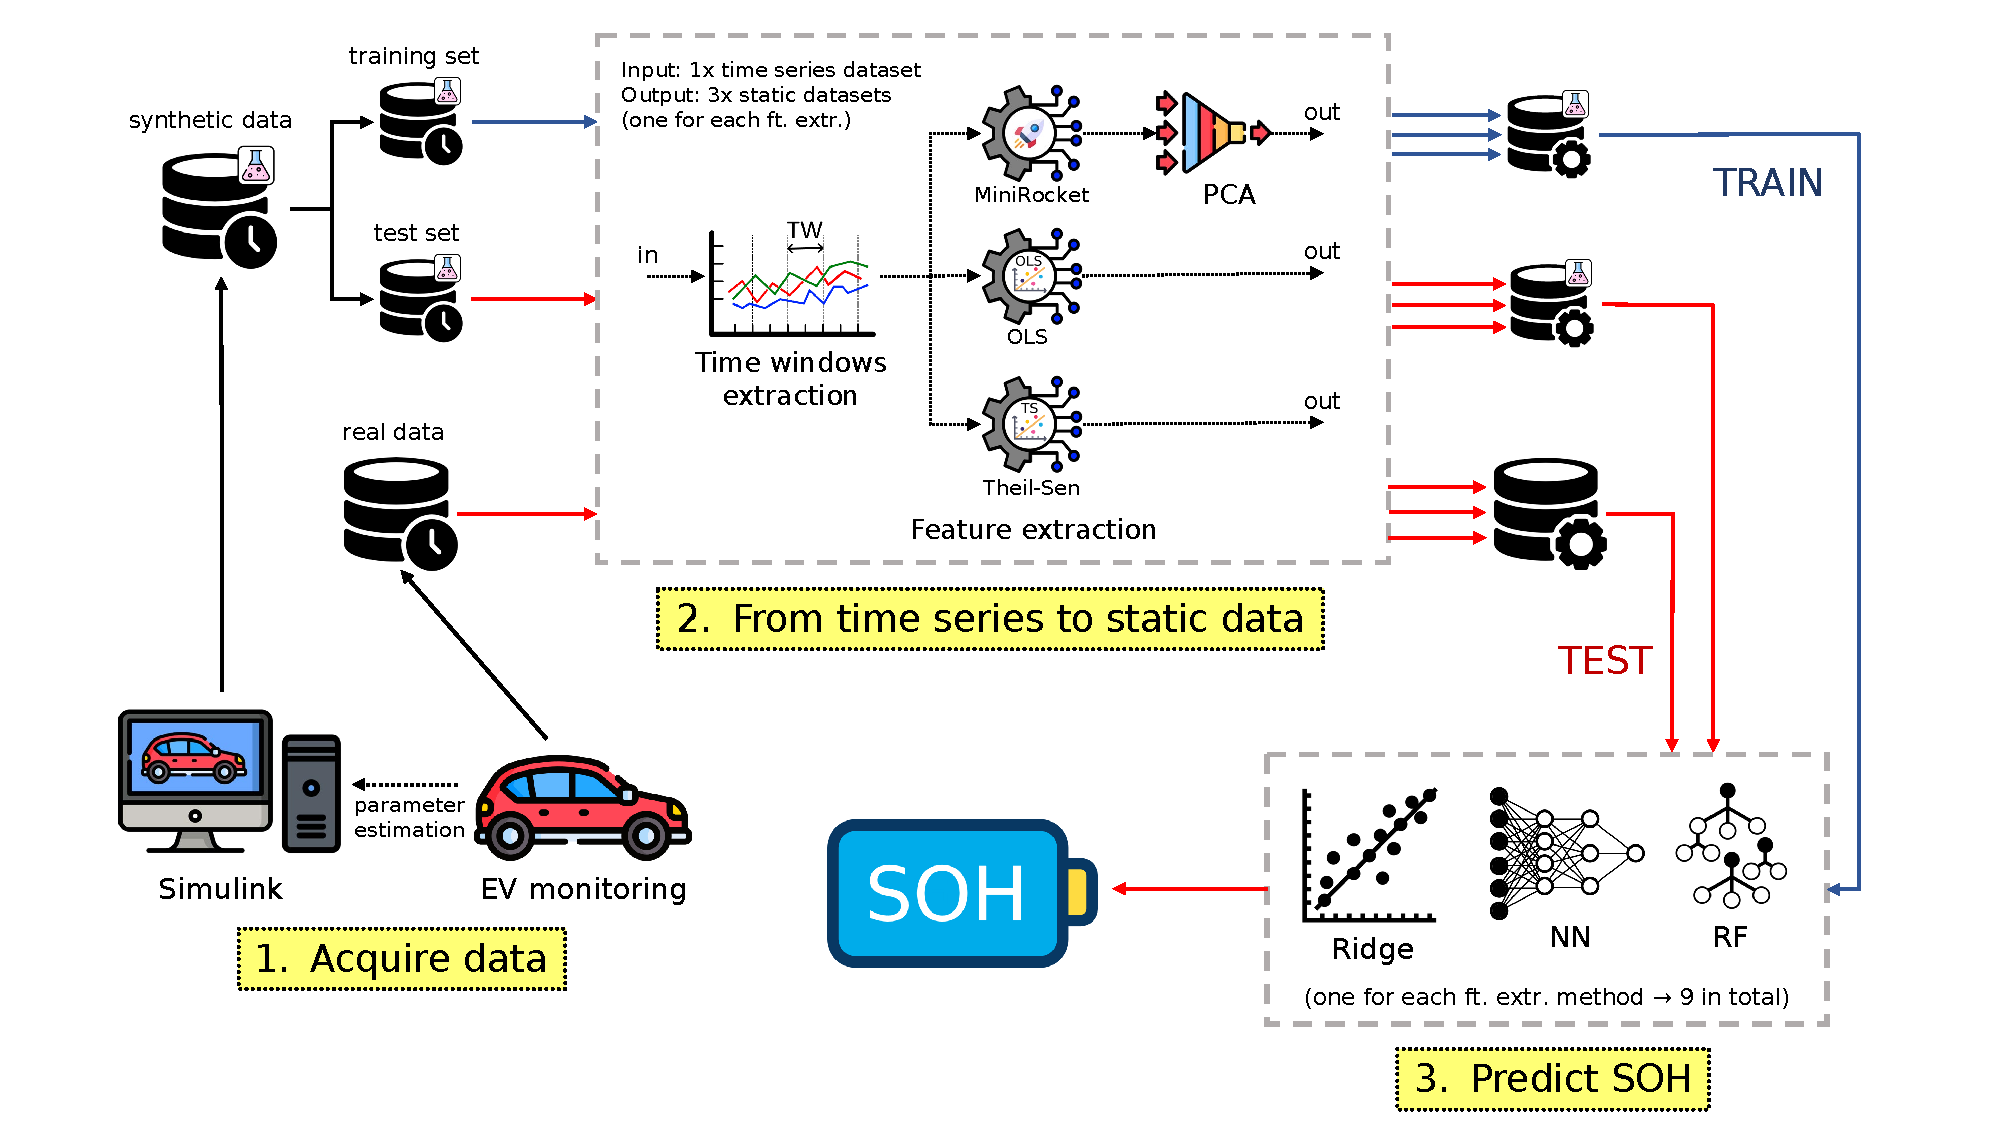
\includegraphics[width=\textwidth]{images/schemone.pdf}
    \caption[Overview of the data pipeline designed to train and test the proposed SOH estimation procedure]{Overview of the data pipeline designed to train and test the proposed SOH estimation procedure.}
    \label{fig:overview}
\end{figure}